\documentclass{beamer}

\usefonttheme{professionalfonts} % using non standard fonts for beamer
\usefonttheme{serif} % default family is serif

%\usepackage{hyperref}

%\usepackage{minted}

\usepackage{animate}

\usepackage{graphicx}

\def\Put(#1,#2)#3{\leavevmode\makebox(0,0){\put(#1,#2){#3}}}

\usepackage{color}

\usepackage{tikz}

\usepackage{amssymb}

\usepackage{enumerate}


\newcommand\blfootnote[1]{%

  \begingroup

  \renewcommand\thefootnote{}\footnote{#1}%

  \addtocounter{footnote}{-1}%

  \endgroup

}

\makeatletter

%%%%%%%%%%%%%%%%%%%%%%%%%%%%%% Textclass specific LaTeX commands.

 % this default might be overridden by plain title style

 \newcommand\makebeamertitle{\frame{\maketitle}}%

 % (ERT) argument for the TOC

 \AtBeginDocument{%

   \let\origtableofcontents=\tableofcontents

   \def\tableofcontents{\@ifnextchar[{\origtableofcontents}{\gobbletableofcontents}}

   \def\gobbletableofcontents#1{\origtableofcontents}

 }

%%%%%%%%%%%%%%%%%%%%%%%%%%%%%% User specified LaTeX commands.

\usetheme{Malmoe}

% or ...

\useoutertheme{infolines}

\addtobeamertemplate{headline}{}{\vskip2pt}



\setbeamercovered{transparent}

% or whatever (possibly just delete it)

\makeatother

\begin{document}
\title[DCEL report]{RIDIR Report}
\author[AC]{Andres Calderon}
\institute[Winter'20]{University of California, Riverside}
\makebeamertitle
\newif\iflattersubsect

\AtBeginSection[] {
    \begin{frame}<beamer>
    \frametitle{Outline} 
    \tableofcontents[currentsection]  
    \end{frame}
    \lattersubsectfalse
}

\AtBeginSubsection[] {
    \begin{frame}<beamer>
    \frametitle{Outline} 
    \tableofcontents[currentsubsection]  
    \end{frame}
}

\begin{frame}{Overlay operator validation}
    \begin{itemize}
        \item For small demos: Visual inspection...
        \item For bigger datasets:
        \begin{enumerate}
            \item Run and extract polygons of the overlay operator from our implementation.
            \item Run and extract polygons of the overlay operator using QGIS.
            \item Run difference operator on the two outputs using QGIS.
            \item If outputs are equal, difference operator must be empty.
        \end{enumerate}
    \end{itemize}
\end{frame}

\begin{frame}{Testing overlay operators: Empty partitions...}
    \centering
	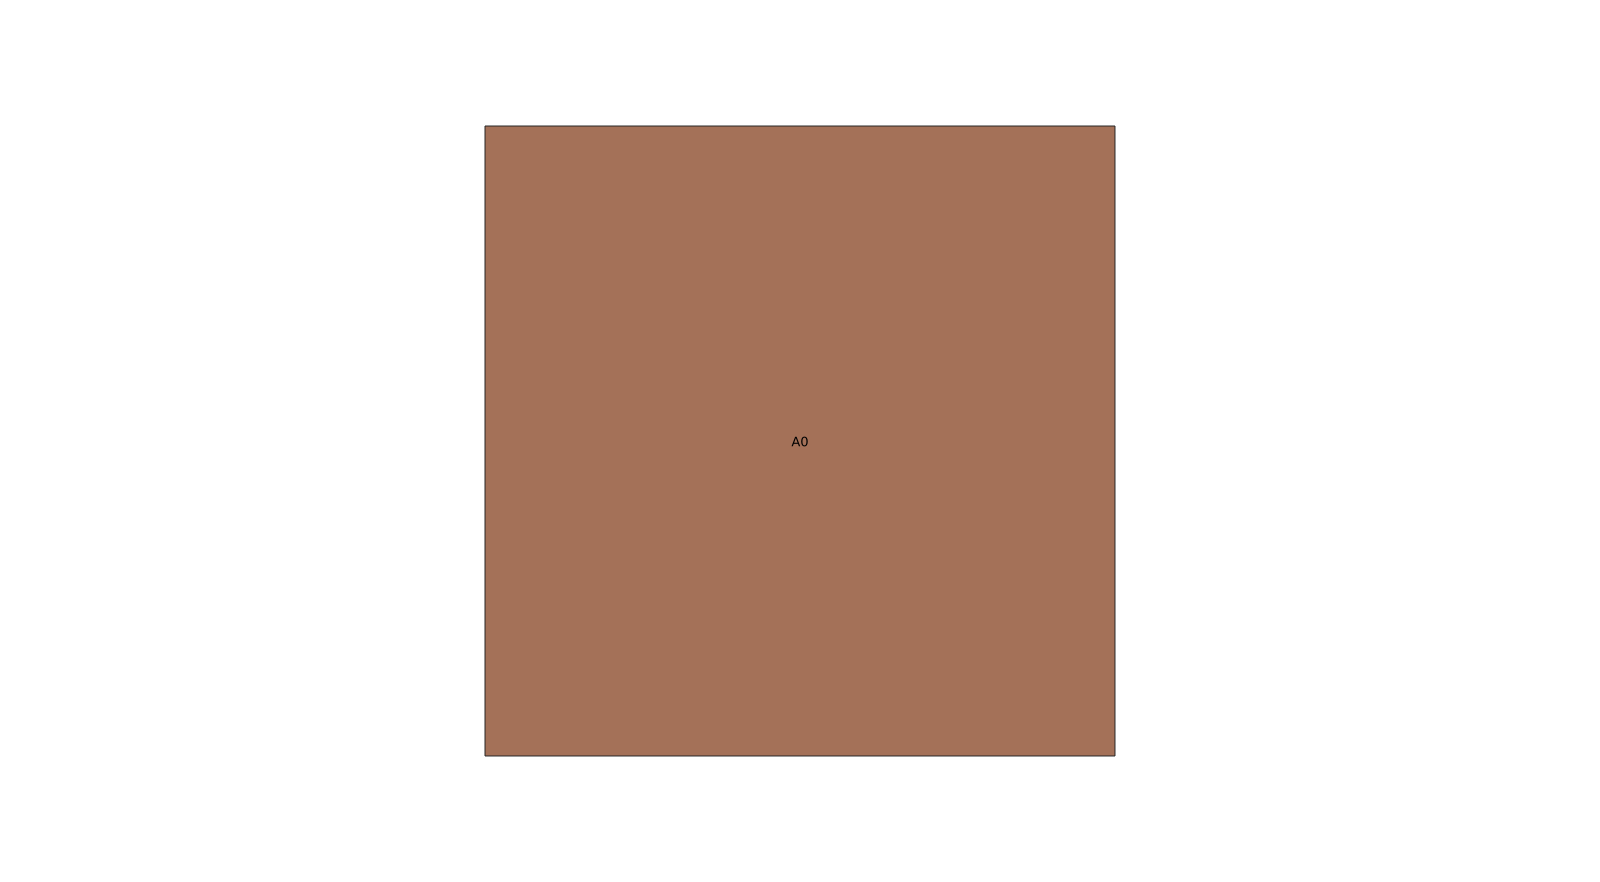
\includegraphics[trim=1cm 0 1cm 0, clip, width=0.9\textwidth]{figures/Demo_A}
\end{frame}
\begin{frame}{Testing overlay operators: Empty partitions...}
    \centering
	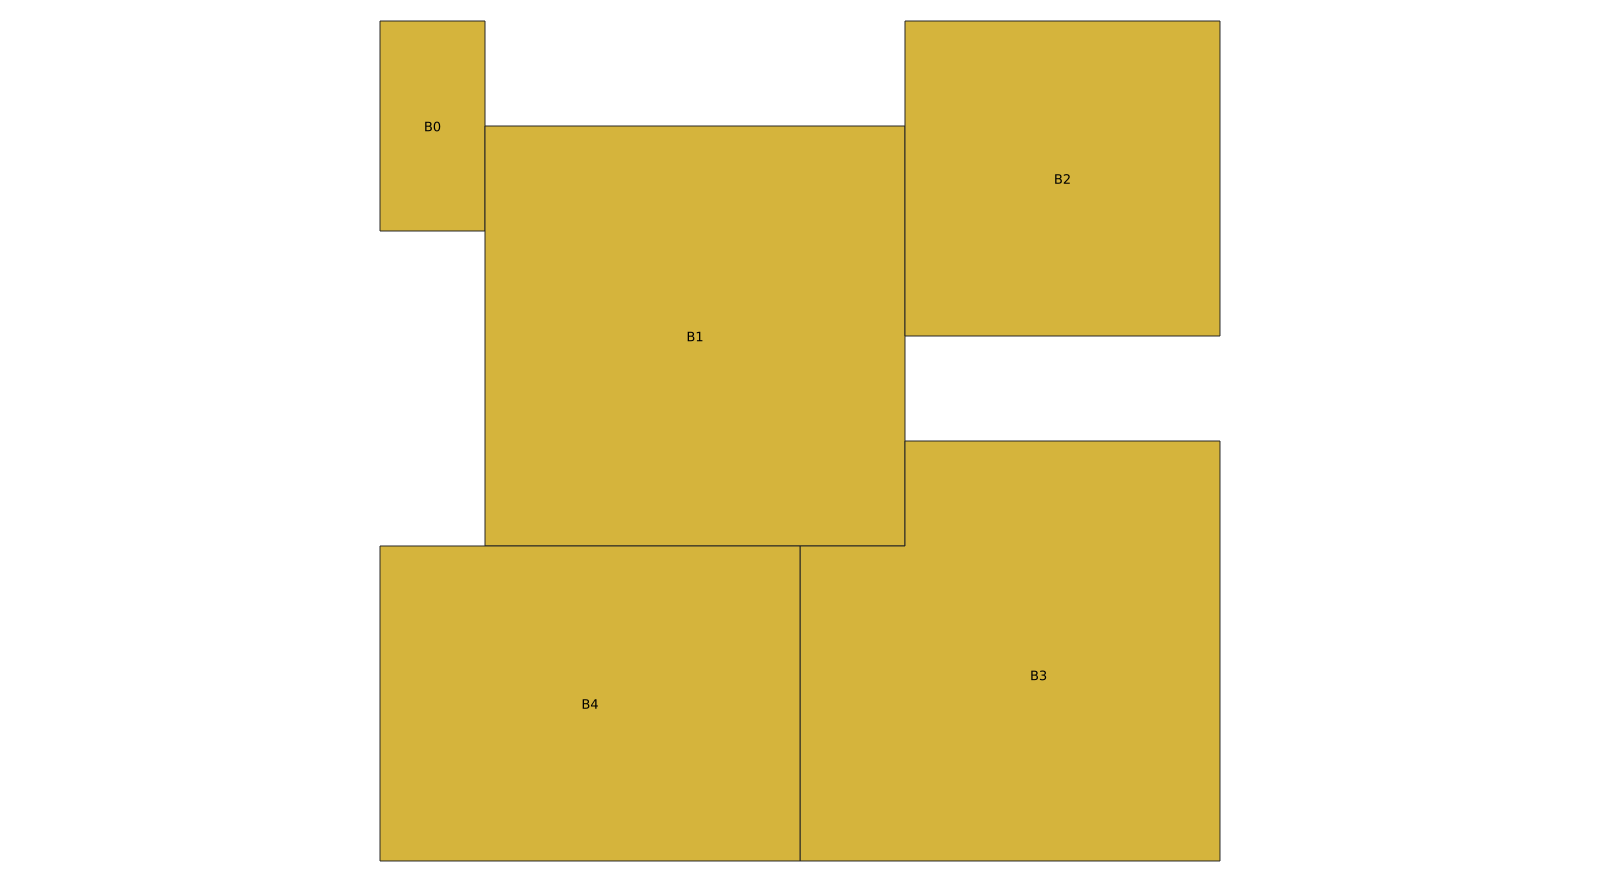
\includegraphics[trim=1cm 0 1cm 0, clip, width=0.9\textwidth]{figures/Demo_B}
\end{frame}
\begin{frame}{Testing overlay operators: Empty partitions...}
    \centering
	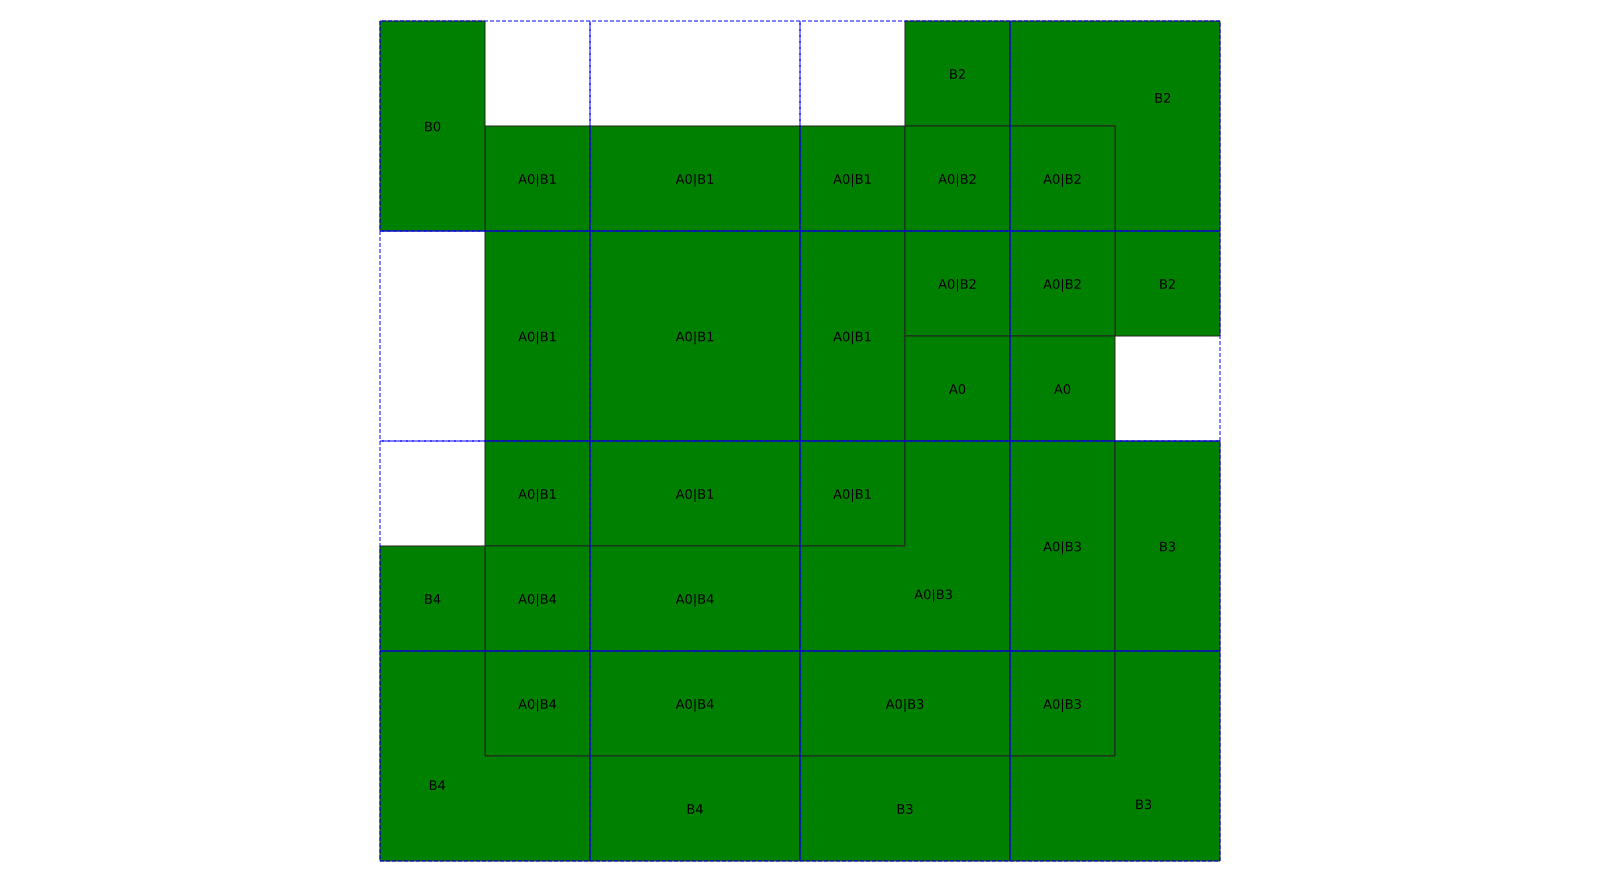
\includegraphics[trim=1cm 0 1cm 0, clip, width=0.9\textwidth]{figures/Demo_Faces}
\end{frame}
\begin{frame}{Testing overlay operators: Empty partitions, Intersections...}
    \centering
	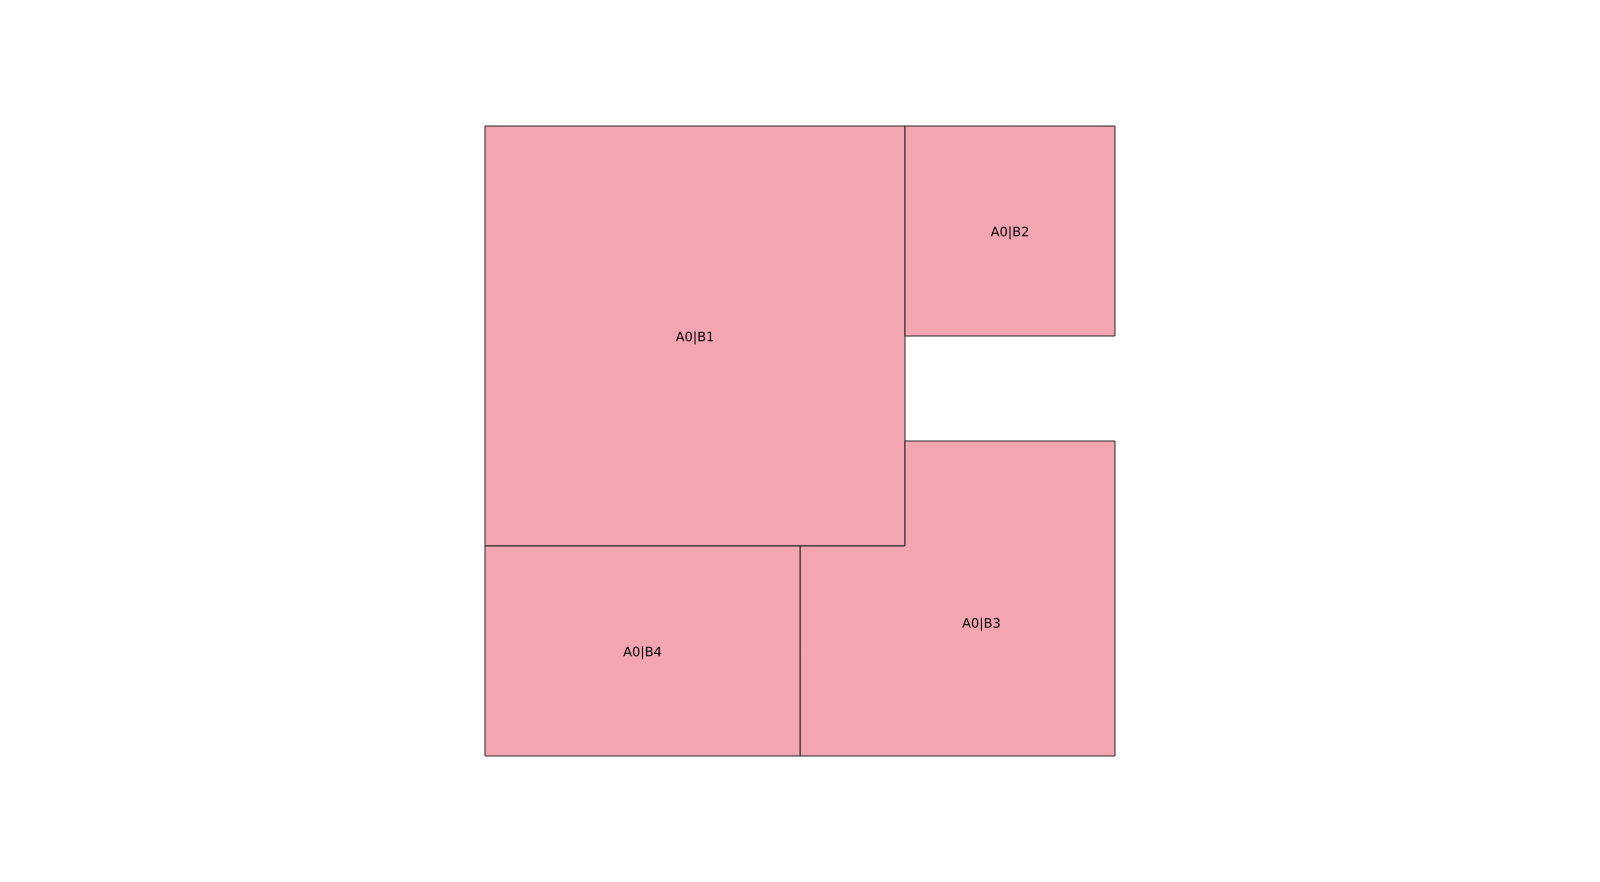
\includegraphics[trim=1cm 0 1cm 0, clip, width=0.9\textwidth]{figures/Demo_Intersection}
\end{frame}
\begin{frame}{Testing overlay operators: Empty partitions, Symmetric difference...}
    \centering
	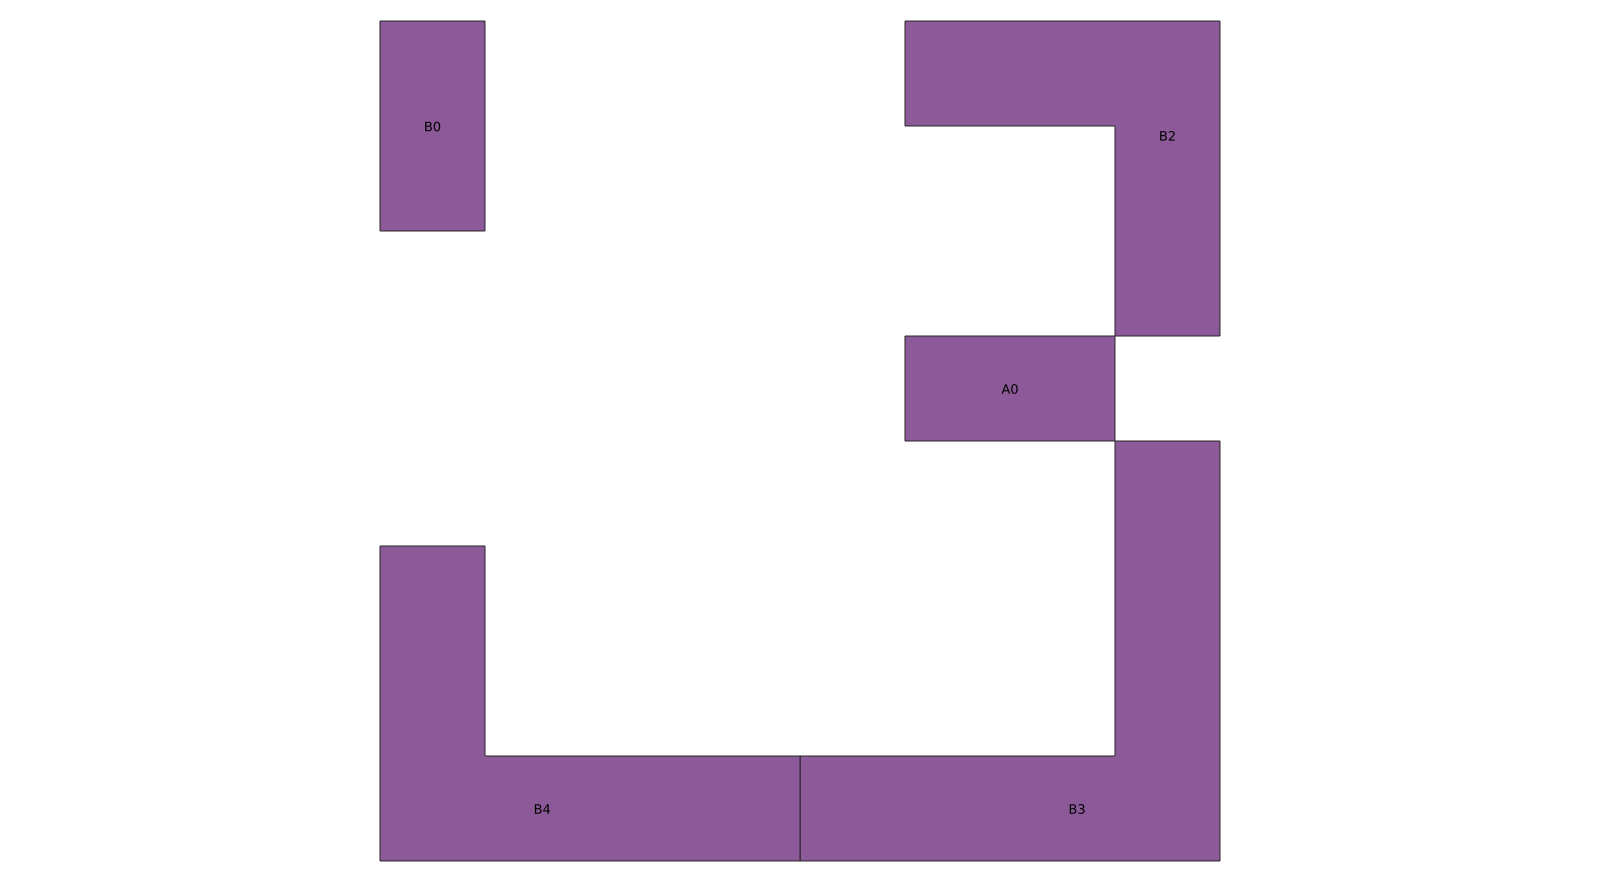
\includegraphics[trim=1cm 0 1cm 0, clip, width=0.9\textwidth]{figures/Demo_Symmetric}
\end{frame}

\begin{frame}{Testing overlay operators: Holes...}
    \centering
	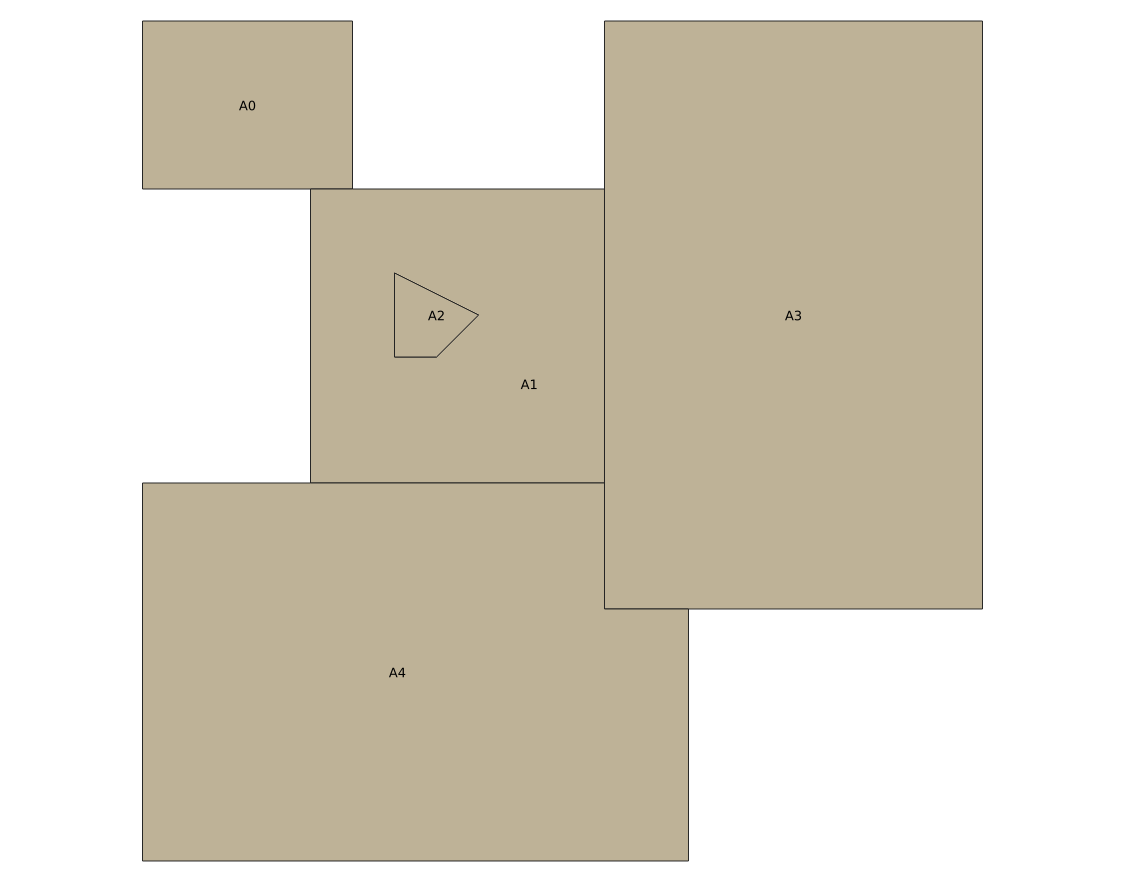
\includegraphics[trim=1cm 0 1cm 0, clip, width=0.8\textwidth]{figures/Holes_A}
\end{frame}
\begin{frame}{Testing overlay operators: Holes...}
    \centering
	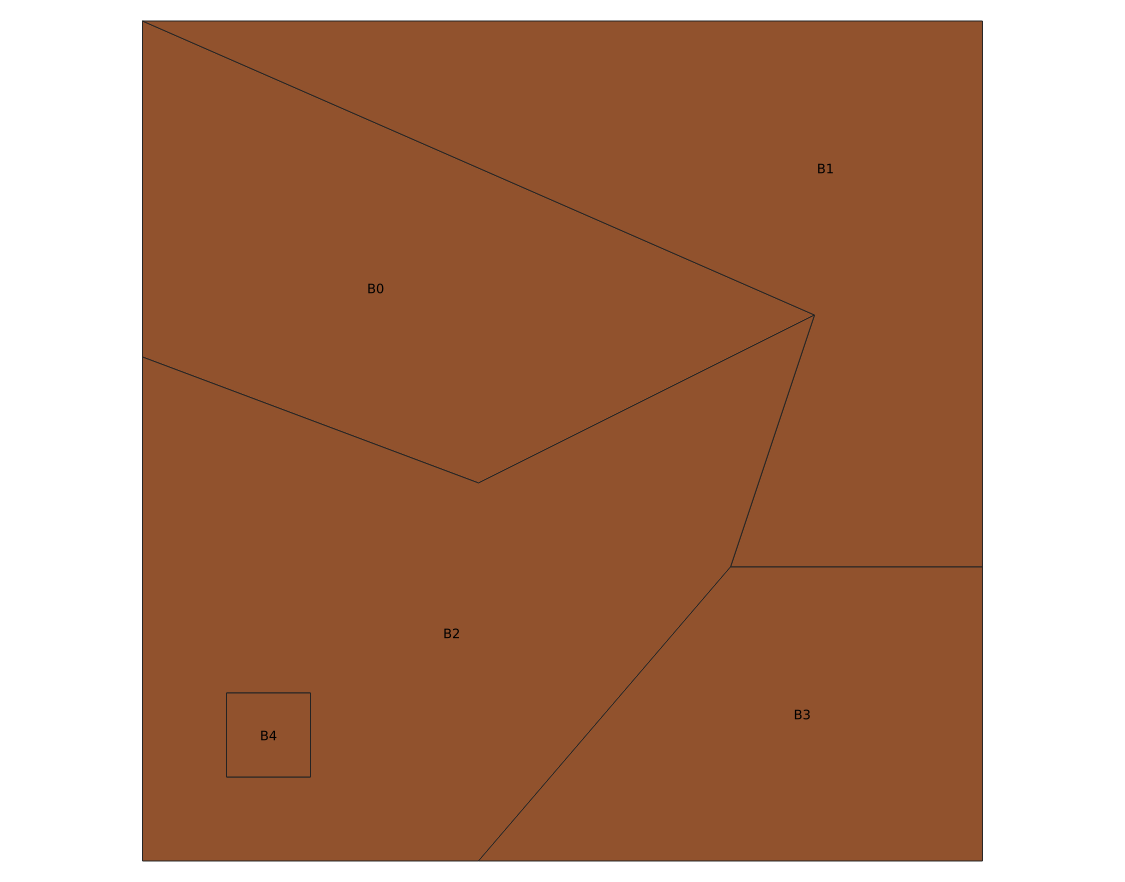
\includegraphics[trim=1cm 0 1cm 0, clip, width=0.8\textwidth]{figures/Holes_B}
\end{frame}
\begin{frame}{Testing overlay operators: Holes...}
    \centering
	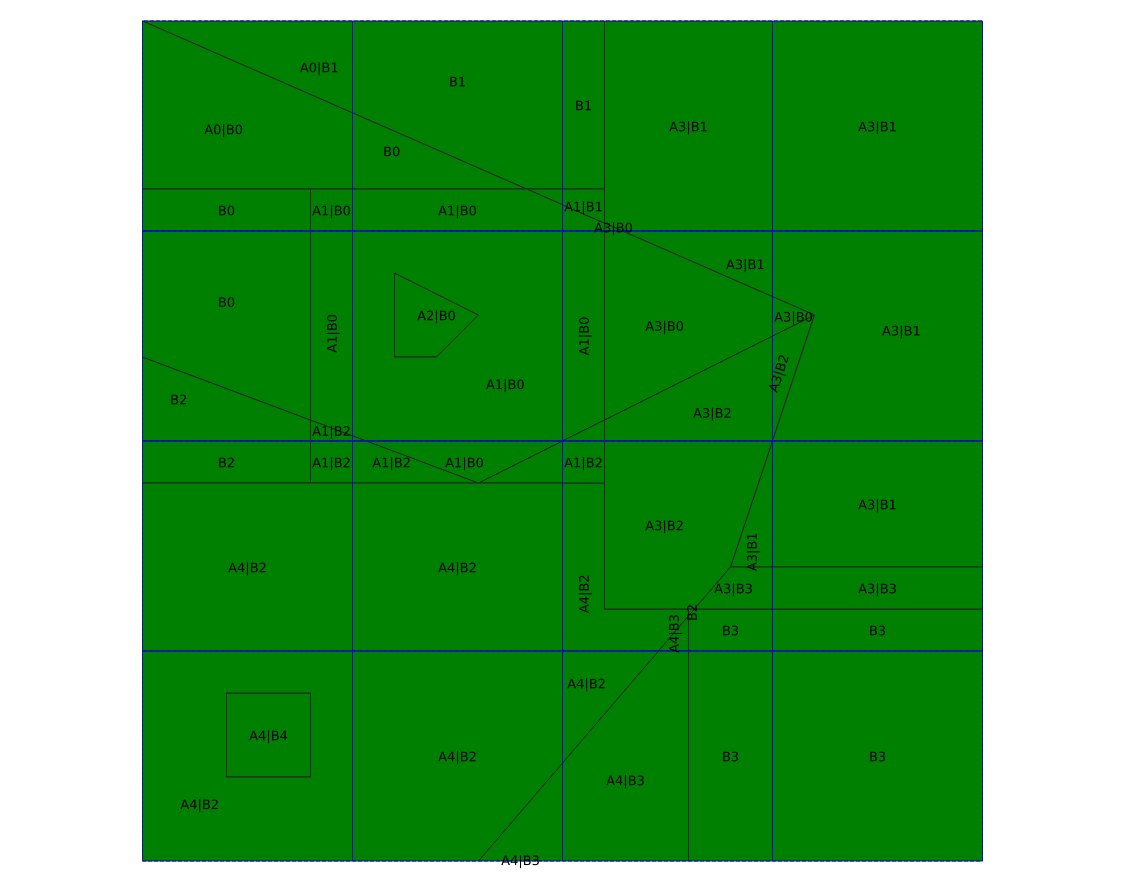
\includegraphics[trim=1cm 0 1cm 0, clip, width=0.8\textwidth]{figures/Holes_Faces}
\end{frame}
\begin{frame}{Testing overlay operators: Holes, Intersections...}
    \centering
	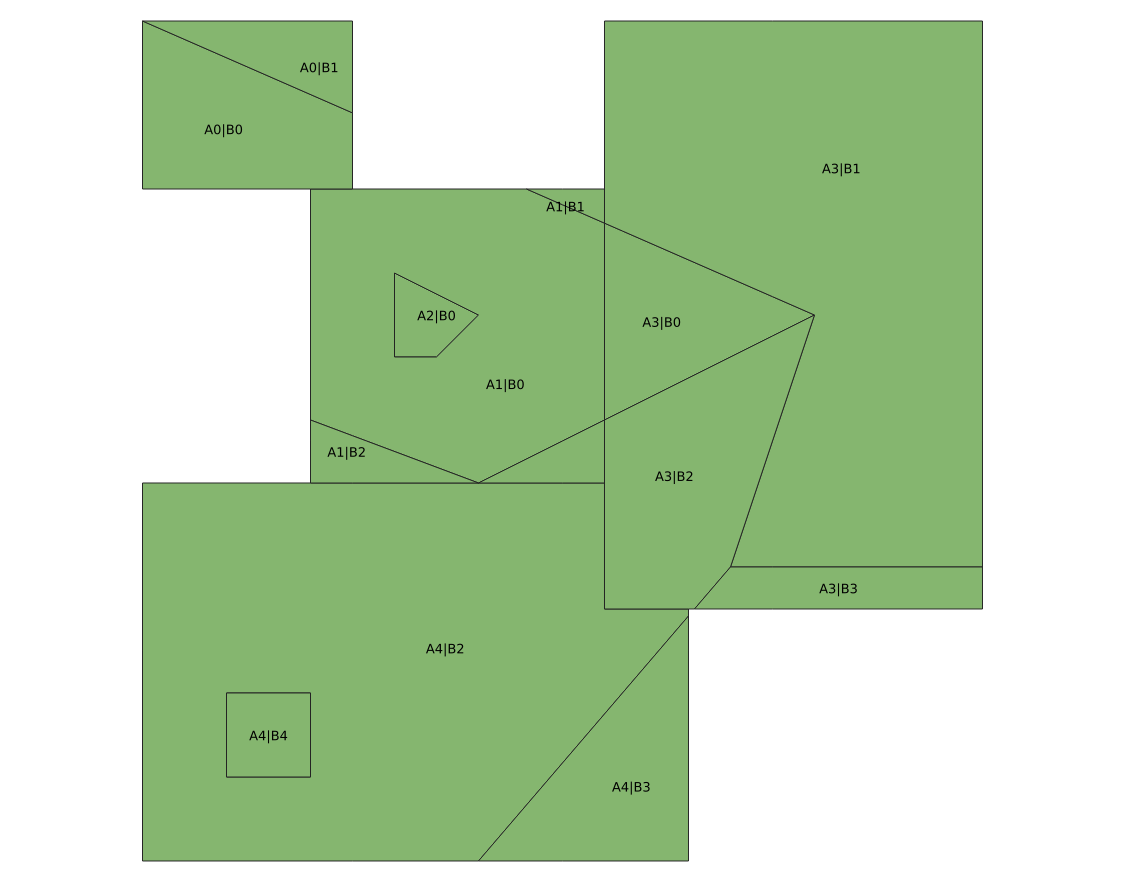
\includegraphics[trim=1cm 0 1cm 0, clip, width=0.8\textwidth]{figures/Holes_Intersection}
\end{frame}
\begin{frame}{Testing overlay operators: Holes, Symmetric difference...}
    \centering
	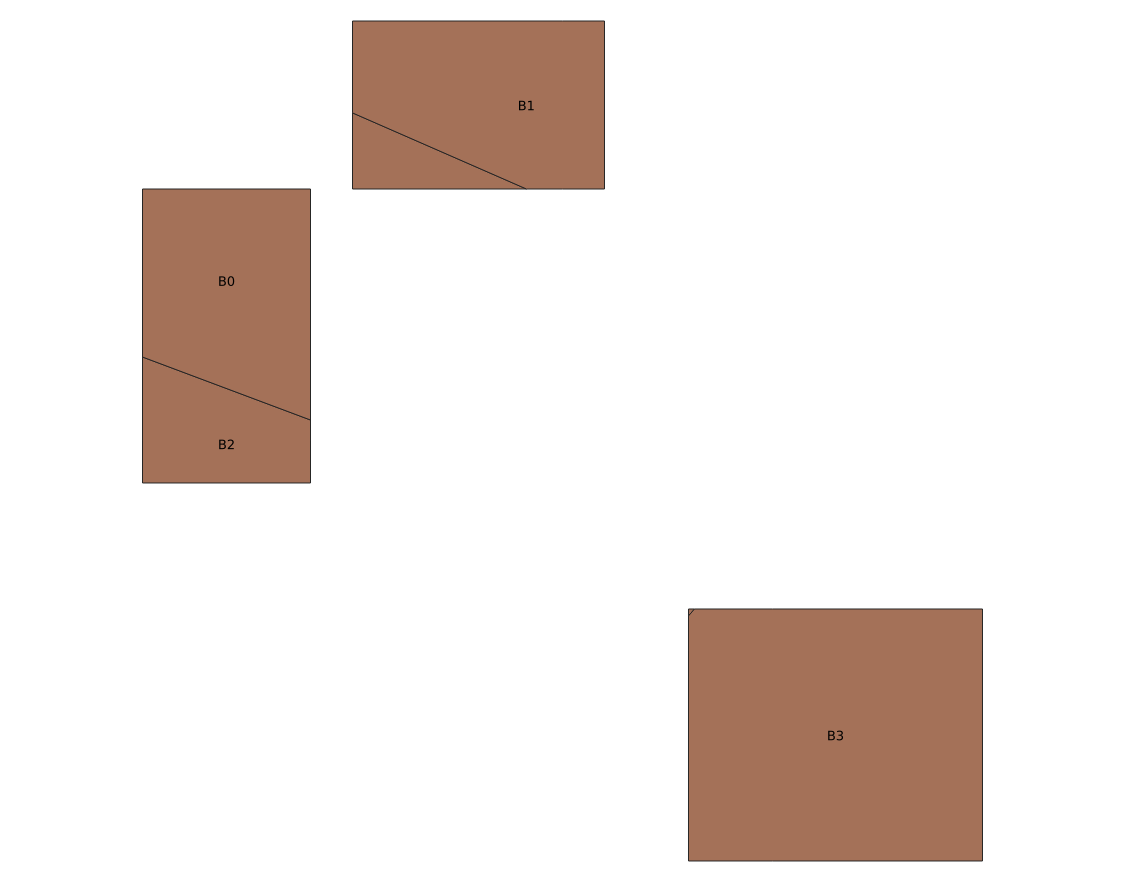
\includegraphics[trim=1cm 0 1cm 0, clip, width=0.8\textwidth]{figures/Holes_Symmetric}
\end{frame}

\begin{frame}{Testing overlay operators: Phili, Faces...}
    \centering
	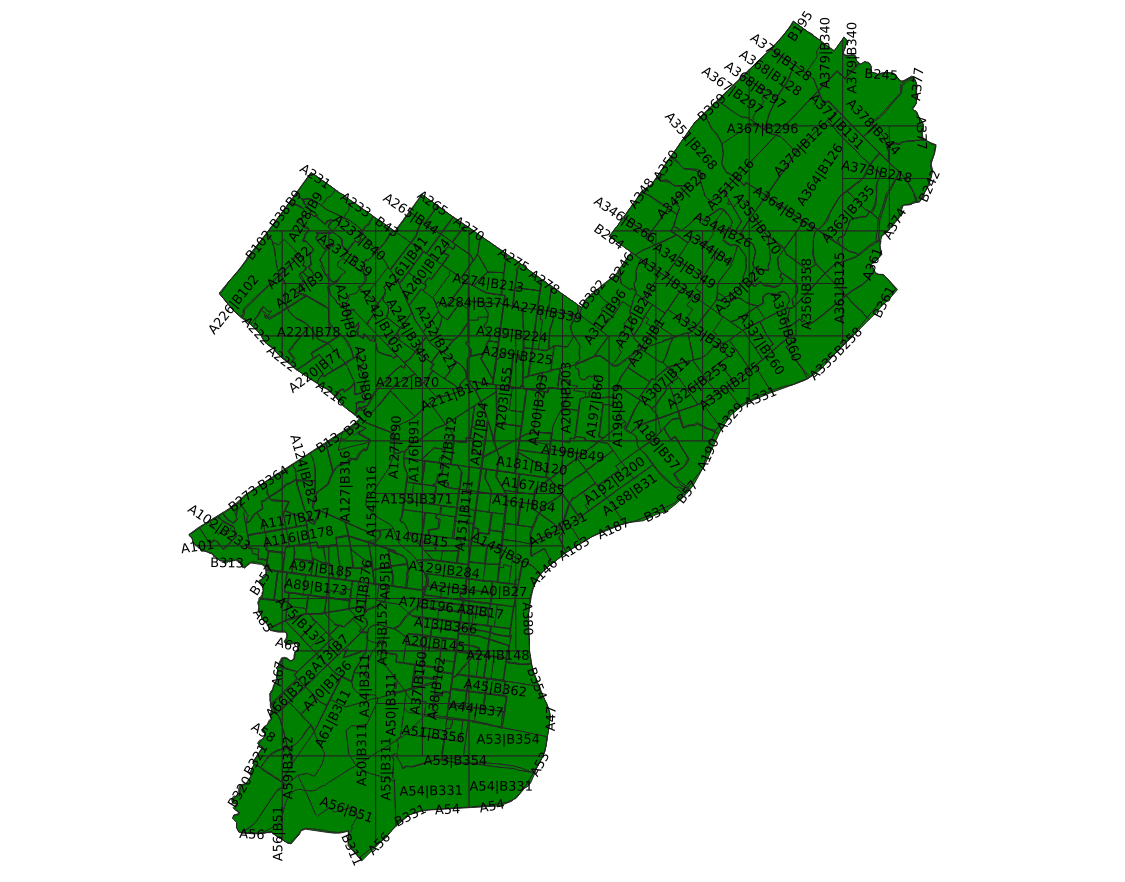
\includegraphics[trim=1cm 0 1cm 0, clip, width=0.8\textwidth]{figures/Phili_Faces}
\end{frame}
\begin{frame}{Testing overlay operators: Phili, Intersections...}
    \centering
	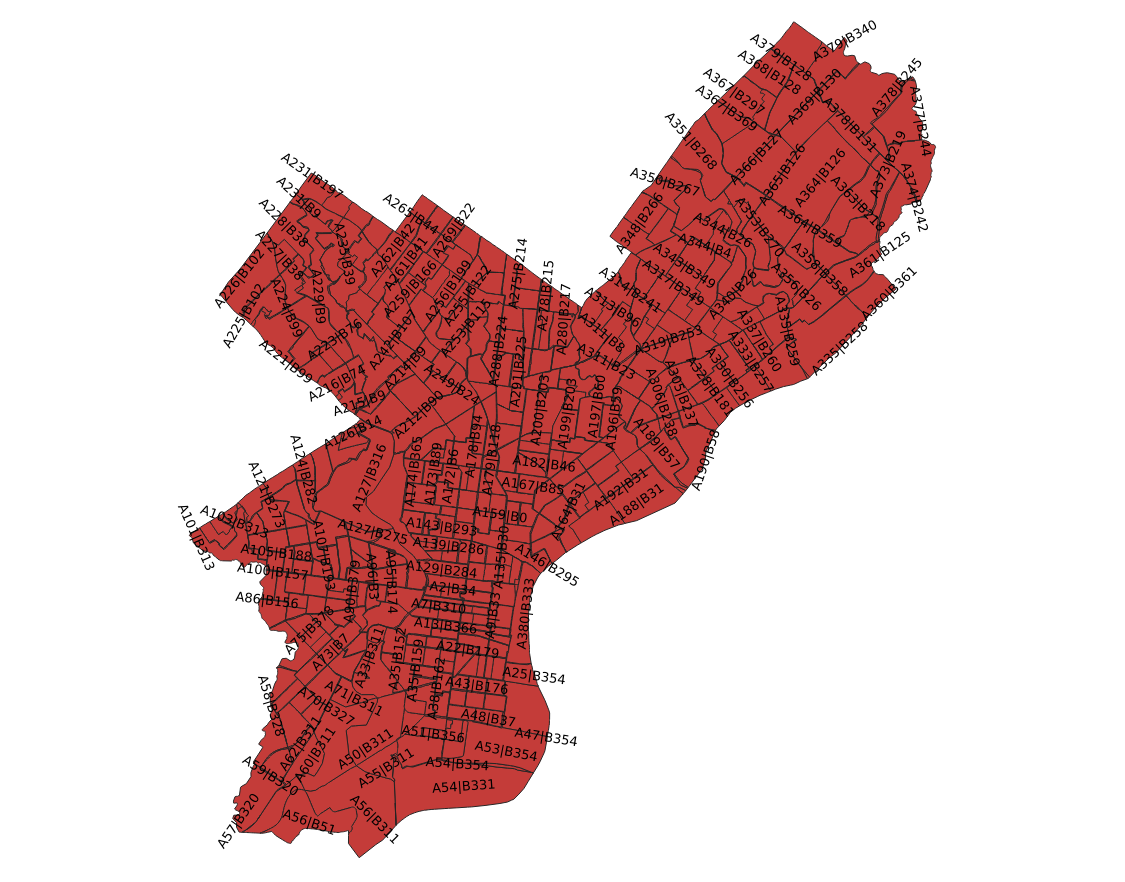
\includegraphics[trim=1cm 0 1cm 0, clip, width=0.8\textwidth]{figures/Phili_Intersections}
\end{frame}
\begin{frame}{Testing overlay operators: Phili, Symmetric difference...}
    \centering
	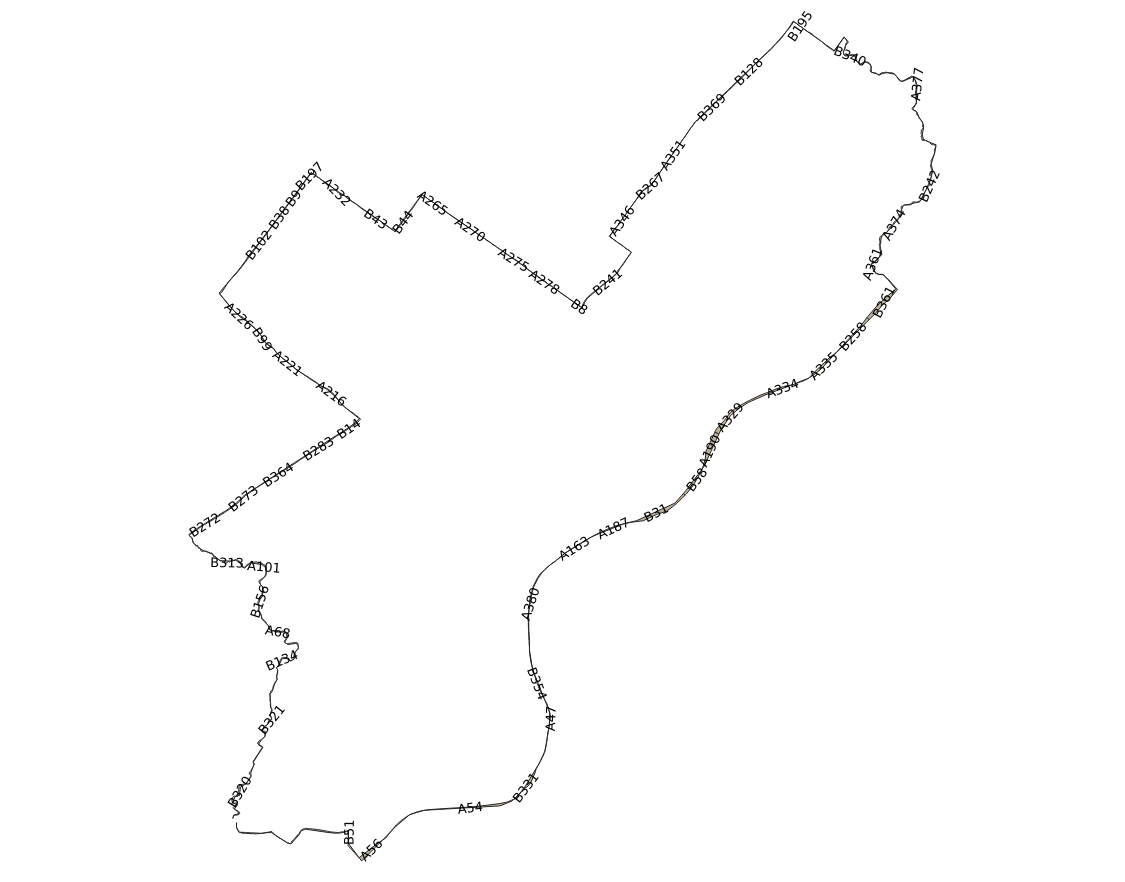
\includegraphics[trim=1cm 0 1cm 0, clip, width=0.8\textwidth]{figures/Phili_Symmetric}
\end{frame}

\begin{frame}{Testing overlay operators: CA, Faces...}
    \centering
	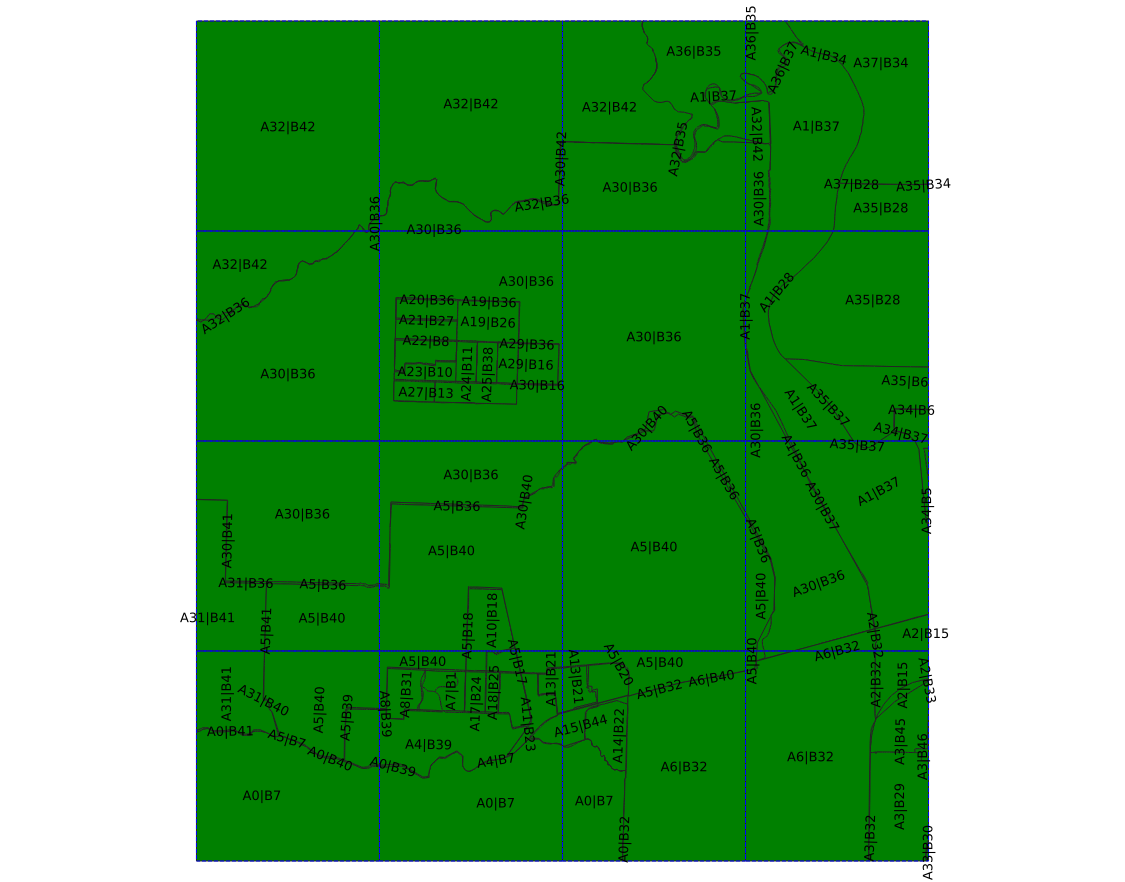
\includegraphics[trim=1cm 0 1cm 0, clip, width=0.8\textwidth]{figures/CA_Faces}
\end{frame}
\begin{frame}{Testing overlay operators: CA, Intersections...}
    \centering
	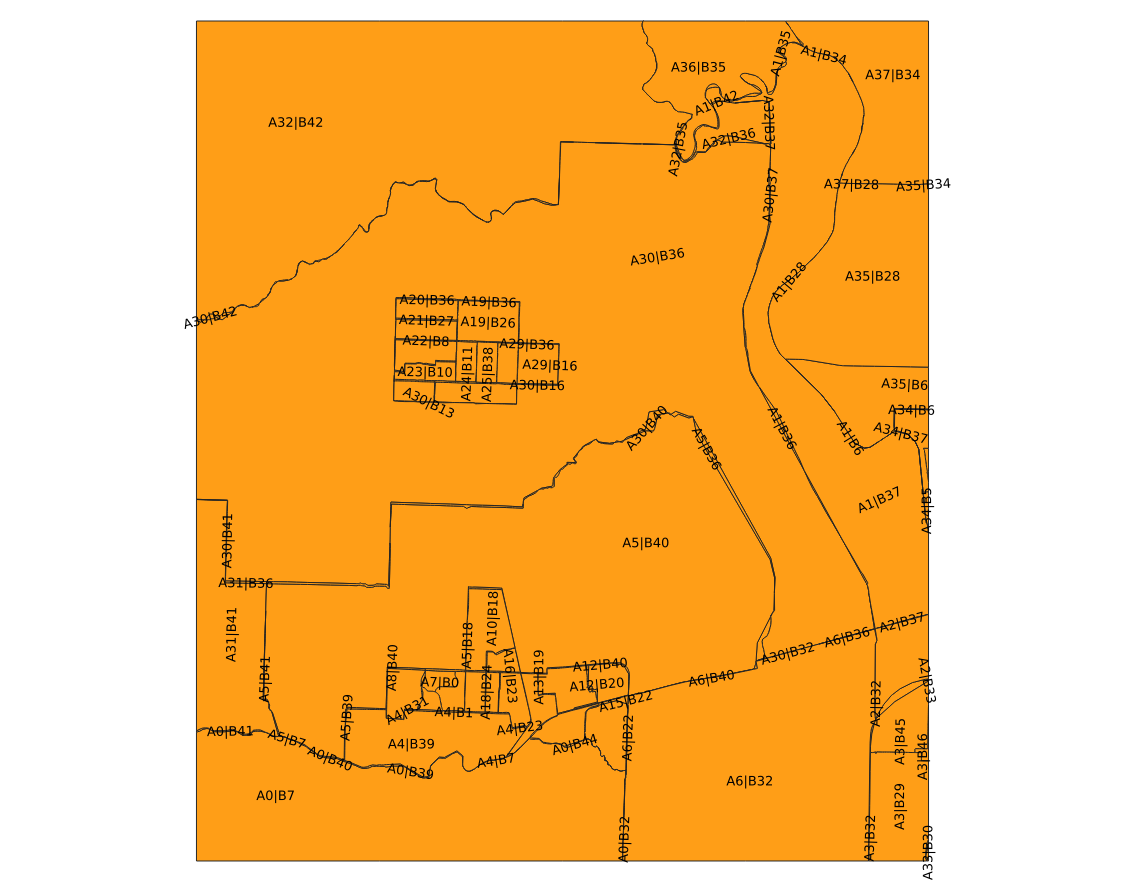
\includegraphics[trim=1cm 0 1cm 0, clip, width=0.8\textwidth]{figures/CA_Intersections}
\end{frame}

\begin{frame}{What's next?}
    \begin{itemize}
        \item I still have a bug at the moment of the merge in the full CA dataset.  Currently working on that...
        \item Tuning cluster parameters...
        \item Benchmarking with sequential tool...
    \end{itemize}
\end{frame}

\end{document}
